\usepackage{amsmath,amssymb}
\usepackage{amsthm}

\usepackage{setspace}
\usepackage{tikz}
\usepackage{mathtools}
\usepackage[francais]{babel}
\uselanguage{French}
\languagepath{French}
\usepackage{pgfplots}
\usepackage{pgfplotstable}
\usepackage{subcaption}
% \newlist{longenumerate}{enumerate}{4}
% \setlist[longenumerate,0]{label=\usebeamerfont*{enumerate item}%
%   \usebeamercolor[fg]{enumerate item}
%   \usebeamertemplate{enumerate item}}
%  
\usepgflibrary{shapes.geometric}
\usetikzlibrary{fit}
\usetikzlibrary{backgrounds}
\usetikzlibrary{positioning} 
%\usetikzlibrary{pgfplots.external}
%\usetikzlibrary{pgfplots.units} 
%\usepgfplotslibrary{external}
\usetikzlibrary{shapes.multipart}
\usetikzlibrary{fit}

\newtheorem{property}{Propriété}

\newcommand{\vect}[1]{ {\boldsymbol {#1}}}
\newcommand{\eye}{1}
\newcommand{\kron}{\bigotimes}

 \beamerdefaultoverlayspecification{}
\setbeamercovered{transparent}

\newenvironment{plusenv}{\alt{\setbeamertemplate{itemize item}{$\textcolor{green}{\oplus}$}}
{\setbeamertemplate{itemize item}{$\textcolor{gray}{\oplus}$}}}{}
\newenvironment{moinsenv}{\alt{\setbeamertemplate{itemize item}{$\textcolor{red}{\ominus}$}}
{\setbeamertemplate{itemize item}{$\textcolor{gray}{\ominus}$}}}{}
\def\plusitem{\item<+-| plus@+-| handout:plus@0-> }
\def\moinsitem{\item<+-| moins@+-| handout:moins@0-> }

\newenvironment{pmenv}{\alt{\setbeamertemplate{itemize item}{$\textcolor{blue}{\pm}$}}
{\setbeamertemplate{itemize item}{$\textcolor{gray}{\pm}$}}}{}
\def\pmitem{\item<+-| pm@+-| handout:pm@0-> }

% \setbeamercolor{section in toc}{fg=red}
% \setbeamercolor{section in toc shaded}{fg=blue}
% 
% \setbeamercolor{subsection in toc}{fg=red}
% \setbeamercolor{subsection in toc shaded}{fg=blue}

\pgfplotsset{compat=1.6}

\title[Navier-Stokes]{Simulation du Jet D'Eau de A à Y:\\ Algorithme numérique pour résoudre les équations de Navier-Stokes incompressibles}


\author{Pablo Strasser}


\institute[Unige] % (optional, but mostly needed)
{University of Geneva}



\date[\today] % (optional, should be abbreviation of conference name)
{\today}

\subject{Navier-Stokes}


\begin{document}
\setlength{\belowdisplayskip}{0pt}%
\setlength{\abovedisplayskip}{0pt}%
\begin{frame}
  \titlepage
\end{frame}

\begin{frame}[shrink]{Résumé}
  \tableofcontents[pausesections]
\end{frame}

\section{Notation et propriété basique}

\begin{frame}{Opérateur différentiel}
Gradient:
\begin{equation*}
 \vect{\nabla}p=\sum_{i}\partial_{i}p
\end{equation*}
Divergence:
\begin{equation*}
 \vect{\nabla}\cdot \vect{v}=\sum_{i}\partial_{i}\vect{v}_{i}
\end{equation*}
Rotationnel
\begin{equation*}
 \vect{\nabla} \times \vect{v}=\begin{pmatrix}
                                \partial_{2}\vect{v}_{3}-\partial_{3}\vect{v}_{2}\\
                                \partial_{3}\vect{v}_{1}-\partial_{1}\vect{v}_{3}\\
                                \partial_{1}\vect{v}_{2}-\partial_{2}\vect{v}_{1}\\
                               \end{pmatrix}
 \end{equation*}

Convection
\begin{equation*}
 \left(\vect{v}\cdot \vect{\nabla}\right)\vect{v}=\sum_{i} \vect{v}_{i}\partial_{i} \vect{v}
 \end{equation*}

\end{frame}
\begin{frame}[<+->]{Propriété des opérateurs différentiels}
 \begin{property}[Divergence d'un rotationnel]
  \begin{equation*}
  \nabla \cdot \left(\nabla \times \vect{v}\right)=0
  \end{equation*}
 \end{property}

 \begin{property}[Rotationnel d'un gradient]
  \begin{equation*}
  \nabla \times \left(\nabla p\right)=0
  \end{equation*}
 \end{property}
\end{frame}

\begin{frame}{Projection}
 
 \begin{property}
 Pour chaque vecteur $\vect{v}$ on peut \emph{projeter} dans un espace à \emph{divergence} nulle sans changer le \emph{rotationnel} en résolvant:
  \begin{align*}
  \vect{v}_{new}&=\vect{v}-\vect{\nabla} p\\
  \Delta p&=\vect{\nabla} \cdot \vect{v}
  \end{align*}
\begin{block}<+->{Preuve}
  
   \begin{align*}
   \uncover<.->{\vect{\nabla}\cdot \vect{v}_{new}}&\uncover<.->{=\vect{\nabla} \cdot \vect{v}-\Delta p=\vect{\nabla} \cdot \vect{v}-\vect{\nabla} \cdot \vect{v}=0
   }\\
   \uncover<+->{
    \vect{\nabla} \times \vect{v}_{new}}&\uncover<.->{=\vect{\nabla} \times \vect{v}-\vect{\nabla}\times \vect{\nabla}p=\vect{\nabla} \times \vect{v}
    }
   \end{align*}
 \end{block}
 \end{property}

  \begin{definition}<+->[Projecteur]
  \begin{equation*}
   P\vect{v}=\vect{\nabla}\Delta^{-1}\vect{\nabla}\cdot \vect{v}
  \end{equation*}
 \end{definition}
 
\end{frame}


\section{Navier-Stokes}
\begin{frame}[<+->]{Reformulation avec projection}
 \begin{block}{Navier-Stokes}
\begin{align*}
\vect{\nabla} \cdot \vect{v}(\vect{x} ,t)&=0\\
\partial_t \vect{v}(\vect{x} ,t)&=\underbrace{f(\vect{v}(\vect{x},t))-\vect{\nabla}p}_{\text{Accélération}}
\intertext{Où}
f(\vect{v}(\vect{x},t))&=-(\vect{v}\cdot\vect{\nabla} ) \vect{v}+\frac{\vect{F}}{\rho}+\nu \Delta \vect{v}
\end{align*}
 \end{block}
 
 \begin{block}{Reformulation}
 \begin{align*}
  \partial_t \left(\vect{\nabla}\cdot \vect{v}\right)&=0=\vect{\nabla}\cdot f(\vect{v})-\Delta p\\
  \Delta p&=\vect{\nabla}\cdot f(\vect{v})\\
  \partial_t \vect{v}&=(1-P)f(\vect{v})
  \end{align*}
 \end{block}


\end{frame}

\begin{frame}[<+->]{Définition lagrangienne}
 \begin{block}{Caracteristique}
\begin{align*}
 \partial_t \vect{\xi}_{\lambda}(t)&=\vect{v}(\vect{\xi}_{\lambda}(t),t)\\
 \vect{\xi}_{\lambda}(t_0)&=\vect{\xi}^{0}_{\lambda}
\end{align*}
\end{block}

\begin{block}{Vitesse lagrangienne}
\begin{equation*}
 \vect{u}_{\lambda}(t)=\vect{v}(\vect{\xi}_{\lambda}(t),t)
\end{equation*}
\end{block}

\begin{block}{Dérivée matérielle}
\begin{align*}
\frac{d \vect{u}_{\lambda}(t)}{d t}&=\frac{d \vect{v}(\xi_{\lambda},t)}{d t}=\partial_t \vect{v}+\left(\frac{\partial \vect{\xi}_{\lambda}(t)}{\partial t}\cdot\vect{\nabla}\right)\vect{v}\\
\frac{d \vect{u}_{\lambda}(t)}{d t}&=\partial_t \vect{v}+\left(\vect{v} \cdot\vect{\nabla}\right)\vect{v}
\end{align*}
 \end{block}

\end{frame}
\begin{frame}{Navier-Stokes lagrangien}
 \begin{block}{Navier-Stokes lagrangien}
 \begin{align*}
\vect{\nabla} \cdot \vect{u}_{\lambda}(t)&=0\\
\frac{d \vect{u}_{\lambda}(t)}{d t}&=-\vect{\nabla} p(\vect{\xi}_{\lambda}(t),t)+\frac{\vect{F}(\vect{\xi}_{\lambda}(t),t)}{\rho(\vect{x},t)}+\nu \Delta \vect{u}_{\lambda}(t)
 \end{align*}
 \end{block}

\end{frame}


\begin{frame}[<+->]{Différentes versions des équations de Navier-Stokes}
 \setlength{\abovedisplayskip}{0pt}
 \setlength{\abovedisplayshortskip}{0pt}
 \begin{block}{Eulerien}
 \begin{align*}
  \vect{\nabla} \cdot \vect{v}(\vect{x} ,t)&=0\\
\partial_t \vect{v}(\vect{x} ,t)&=f(\vect{v}(\vect{x},t))-\vect{\nabla}p
\end{align*}
 \end{block}
 \begin{block}{Projection}
 \begin{equation*}
  \partial_t \vect{v}=(1-P)f(\vect{v})
  \end{equation*}
 \end{block}

 \begin{block}{Lagrangien}
  \begin{align*}
\vect{\nabla} \cdot \vect{u}_{\lambda}(t)&=0\\
\frac{d \vect{u}_{\lambda}(t)}{d t}&=-\vect{\nabla} p(\vect{\xi}_{\lambda}(t),t)+\frac{\vect{F}(\vect{\xi}_{\lambda}(t),t)}{\rho(\vect{x},t)}+\nu \Delta \vect{u}_{\lambda}(t)
 \end{align*}
 \end{block}


\end{frame}

\section{Projection}
\begin{frame}[<+->]{Idée}
 \begin{itemize}
  \item Vitesse et pression sont discrétisées sur une grille.
  \item Les équations de Navier-Stokes sont résolues sur la grille.
  \item Mais la topologie est determinée par la position des particules.
  \item Les particules se déplacent par la vitesse donnée par interpolation de la grille.
  \item Les conditions aux bords sont imposées en créant des points fantômes en vitesse et pression
 \end{itemize}

\end{frame}
\begin{frame}[fragile]{Schéma de l'algorithme}
\shorthandoff{:;}
 \begin{tikzpicture}[scale=1,node distance=4mm,line width=0.5mm]
  \node[draw](init)  {Initialisation};
  \node[below= of init,draw](runginit) {Initialisation};
  \node[below= of runginit,draw](extrap) {Extrapolation};
  \node[below= of extrap,draw](gravity) {Gravité};
   \node[below= of gravity,draw](conv) {Convection};
   \node[below= of conv,draw](viscosity) {Viscosité};
   \node[below= of viscosity,draw](projection) {Projection};
   \node[below= of projection,draw](extrapolation) {Extrapolation};
   \node[left= 1.5 of gravity,draw](part){Mouvements des particules};
   \node[draw,fit=(conv) (gravity) (viscosity) (projection) (extrapolation),label={180:{\rotatebox{90}{Accélération}}}](accel) {};
   \node[draw,fit=(accel) (part) (runginit),label={below:Runge-Kutta}] {};
   \draw[->] (init)--(runginit);
   \draw[->] (runginit)--(extrap);
   \draw[->] (extrap)--(gravity);
   \draw[->] (gravity)--(conv);
   \draw[->](conv)--(viscosity);
   \draw[->](viscosity)--(projection);
   \draw[->] (projection)--(extrapolation);
   \draw[->] (extrap)--(part);
 \end{tikzpicture}
 \shorthandon{:;}
\end{frame}
\begin{frame}[<+->]{Projection}
\begin{block}{Projection en accélération}
\begin{equation*}
 \partial_t \vect{v}=(1-P)f(\vect{v})
 \end{equation*}
\end{block}

\begin{block}{Projection en vitesse}
\begin{align*}
 \partial_t \vect{\tilde{v}}&=f(\vect{v})\\
 \vect{v}&=(1-P)\vect{\tilde{v}}
 \end{align*}
\end{block}
 
\end{frame}

\begin{frame}[<+->]{Intégration}
 \begin{block}{Runge-Kutta sur l'accélération}
   \begin{align*}
	\vect{v}_{n+1}&=\vect{v}_{n}+\sum_{i=1}^{s}b_{i}\vect{k}_{i}\\
	\vect{k}_{i}&=\Delta t (1-P)f\left(\vect{v}_{n}+\sum_{j=1}^{s}a_{ij}\vect{k}_{j}\right)
\end{align*}
 \end{block}
 
  \begin{block}{Runge-Kutta sur la vitesse}
   \begin{align*}
\vect{\tilde{v}}_{n+1}&=(1-P)\left(\vect{\tilde{v}}_{n}+\sum_{i=1}^{s}b_{i}\vect{\tilde{k}}_{i}\right)\\
\vect{\tilde{k}}_{i}&=\Delta t f\left((1-P)\left(\vect{\tilde{v}}_{n}+\sum_{j=1}^{s}a_{ij}\vect{\tilde{k}}_{j}\right)\right)
\end{align*}
 \end{block}
\end{frame}
\begin{frame}{Équivalence}
 \begin{theorem}
Si $\vect{v}_{n}=\vect{\tilde{v}}_{n}$ et $\vect{v}_n$ sont à divergence nulle alors $\vect{v}_{n+1}=\vect{\tilde{v}}_{n+1}$.
 \end{theorem}
 
\begin{corollary}
En résolvant l'équation de Navier-Stokes par une méthode de Runge-Kutta, on est éxactement à divergence nulle.
\end{corollary}
\end{frame}


\section{Discrétisation spatial}
\begin{frame}{Discrétisation ``standard''}
\begin{block}{Position des variables}
\shorthandoff{;:} 
\directlua{dofile('unstaggered.lua')}
\shorthandon{:;}
\end{block}
\begin{block}{Dérivée}
 \begin{align*}
  \partial_x a_i&=\frac{a_{i+1}-a_{i-1}}{\Delta x}
  \vect{\nabla} \cdot \vect{v}_{i,j}&=\frac{v^{x}_{i+1,j}-v^{x}_{i-1,j}}{\Delta x}+\frac{v^{y}_{i+1,j}-v^{y}_{i-1,j}}{\Delta y}
\end{align*}
\end{block}
\end{frame}

\begin{frame}{Problème damier}
\begin{alertblock}{Divergence nulle!!!!}
 \directlua{dofile('unstaggered_div2.lua')}
\end{alertblock}

\begin{block}{Solution:}
 Changer la grille.
\end{block}


 
\end{frame}

\begin{frame}{Discrétisation sur grille décalée}
\begin{block}{Position des variables}
\shorthandoff{;:} 
 \directlua{dofile('staggered.lua')}
 \shorthandon{:;}
\end{block}

 
\end{frame}

\begin{frame}{Dérivée sur grill décalée}
\begin{block}{Gradient}
 \begin{equation*}
  \vect{\nabla}p_{ij}=\begin{pmatrix}
    \frac{p_{i,j}-p_{i-1,j}}{\Delta x}\\
    \frac{p_{i,j}-p_{i,j-1}}{\Delta y}\\
                      \end{pmatrix}
 \end{equation*}
\end{block}

\begin{block}{Divergence}
 \begin{equation*}
\vect{\nabla}\cdot \vect{v}_{i,j}=\frac{{v_{x}}_{i+1,j}-{v_{x}}_{i,j}}{\Delta x}+\frac{{v_{y}}_{i,j+1}-{v_{y}}_{i,j}}{\Delta y}
 \end{equation*}
\end{block}
 
 \begin{block}{Laplacien}
 \begin{equation*}
    \Delta p_{i,j}=\frac{p_{i+1,j}-2p_{i,j}+p_{i-1,j}}{(\Delta x)^2}+\frac{p_{i,j+1}-2p_{i,j}+p_{i,j-1}}{(\Delta y)^2}
   \end{equation*}
 \end{block}

 
\end{frame}

\begin{frame}{Terme convectif sur grille décalée}
\begin{block}{Sorte de terme}
 \begin{equation*}
v^{j}\partial_{j}v^{i}
\end{equation*}
\end{block}
\begin{alertblock}{Problème:}
 \directlua{dofile('staggered_convection_upwind.lua')}
\end{alertblock}

\end{frame}

\begin{frame}{Terme convectif sur grille décalée (suite)}
\begin{block}{Dérivée centrée}
 \begin{equation*}
\left(v^{j}\partial_{j}v^{i}\right)^{i}_{\vect{k}}={v^{ji}}_{\vect{k}}\frac{{v^{i}}_{\vect{k}+\vect{e}_j}-{v^{i}}_{\vect{k}-\vect{e}_j}}{2\Delta x_{j}}
\end{equation*}
\end{block}

\begin{block}{Dérivée upwind}
 \setlength{\abovedisplayskip}{-1pt}
 \setlength{\abovedisplayshortskip}{-1pt}
  \setlength{\belowdisplayskip}{-1pt}
 \setlength{\belowdisplayshortskip}{-1pt}
 \begin{align*}
\shortintertext{si ${v^{ji}}_{\vect{k}}<0$}
\left(v^{j}\partial_{j}v^{i}\right)^{i}_{\vect{k}}&={v^{ji}}_{\vect{k}}\frac{{v^{i}}_{\vect{k}+\vect{e}_j}-{v^{i}}_{\vect{k}}}{\Delta x_{j}}\\
\shortintertext{si ${v^{ji}}_{\vect{k}}>0$}
\left(v^{j}\partial_{j}v^{i}\right)^{i}_{\vect{k}}&={v^{ji}}_{\vect{k}}\frac{{v^{i}}_{\vect{k}}-{v^{i}}_{\vect{k}-\vect{e}_j}}{\Delta x_{j}}\\
\shortintertext{si ${v^{ji}}_{\vect{k}}=0$}
\left(v^{j}\partial_{j}v^{i}\right)^{i}_{\vect{k}}&=0
\end{align*}
\end{block}

\end{frame}

\begin{frame}[<+->]{Algorithme en topologie fixe}
 \begin{block}{Principe}
  \begin{itemize}
   \item<1-> Utiliser une méthode de Runge-Kutta de notre choix.
   \item Evaluer l'accéleration sur une ``staggered grid''.
   \item Projeter chaque accélération ou chaque vitesse.
  \end{itemize}
 \end{block}

\begin{block}{Runge-Kutta sur l'accélération}
	\begin{align*}
	\textstyle\vect{v}_{n+1}&\textstyle=\vect{v}_{n}+\sum_{i=1}^{s}b_{i}\vect{k}_{i}\\
	\textstyle\vect{k}_{i}&\textstyle=\Delta t (1-P)f(\vect{v}_{n}+\sum_{j=1}^{s}a_{ij}\vect{k}_{j})
	\end{align*}
\end{block}
 
\begin{block}{Runge-Kutta sur la vitesse}
	\begin{align*}
	\textstyle\vect{\tilde{v}}_{n+1}&\textstyle=(1-P)(\vect{\tilde{v}}_{n}+\sum_{i=1}^{s}b_{i}\vect{\tilde{k}}_{i})\\
	\textstyle\vect{\tilde{k}}_{i}&\textstyle=\Delta t f((1-P)(\vect{\tilde{v}}_{n}+\sum_{j=1}^{s}a_{ij}\vect{\tilde{k}}_{j}))
	\end{align*}
\end{block}
\end{frame}

\begin{frame}[fragile]{Schéma de l'algorithme}
\shorthandoff{:;}
 \begin{tikzpicture}[node distance=4mm,line width=0.5mm]
  \node[draw](init)  {Initialisation};
  \node[below= of init,draw,gray](runginit) {Initialisation};
  \node[below= of runginit,draw,gray](extrap) {Extrapolation};
  \node[below= of extrap,draw,red](gravity) {Gravité};
   \node[below= of gravity,draw,red](conv) {Convection};
   \node[below= of conv,draw,red](viscosity) {Viscosité};
   \node[below= of viscosity,draw,red](projection) {Projection};
   \node[below= of projection,draw](extrapolation) {Extrapolation};
   \node[left= 1.5 of gravity,draw,gray](part){Mouvements des particules};
   \node[draw,fit=(conv) (gravity) (viscosity) (projection) (extrapolation),label={[red]180:{\rotatebox{90}{Accélération}}},red](accel) {};
   \node[draw,red,fit=(accel) (part) (runginit),label={[red]below:Runge-Kutta}] {};
   \draw[->] (init)--(runginit);
   \draw[->] (runginit)--(extrap);
   \draw[->] (extrap)--(gravity);
   \draw[->] (gravity)--(conv);
   \draw[->](conv)--(viscosity);
   \draw[->](viscosity)--(projection);
   \draw[->](projection)--(extrapolation);
   \draw[->] (extrap)--(part);
 \end{tikzpicture}
 \shorthandon{:;}
\end{frame}

\section{Topologie}
\begin{frame}[<+->]{Détermination analytique de la topologie}

\begin{block}{Déplacement de la position}
 \begin{equation*}
  \partial_t\vect{x}=\vect{v}
 \end{equation*}
\end{block}

\begin{block}<*>{Surface libre}
\uncover<+->{
\begin{align*}
	\sigma_{ij}&=-p \delta_{ij}+\nu\left(\frac{\partial v_{i}}{\partial x_{j}}+\frac{\partial v_{j}}{\partial x_{i}}\right)\\
	\textstyle\sum_{i,j}\sigma_{ij}n_{i}n_{j}&=0\\
	\textstyle\sum_{i,j}\sigma_{ij}t^{1}_{i}n_{j}&=0\\
	\textstyle\sum_{i,j}\sigma_{ij}t^{2}_{i}n_{j}&=0
\end{align*}
}
\uncover<+->{
\begin{align*}
 p_{surf}&=A\vect{v}_{int}\\
 \vect{v}_{surf}&=B\vect{v}_{int}
\end{align*}
}
\end{block}
 
\end{frame}

\begin{frame}[<+->]{Discrétisation}

\begin{block}{Chose nécessaire}
 \begin{itemize}
  \item<0-> Résoudre:
  \begin{equation*}
   \dot{\vect{x}}=\vect{v}
  \end{equation*}
  \item Imposer les conditions aux bords variables:
   \begin{align*}
 p_{surf}&=A\vect{v}_{int}\\
 \vect{v}_{surf}&=B\vect{v}_{int}
\end{align*}
 \end{itemize}
 \end{block}

\end{frame}

\begin{frame}[<+->]{Discrétisation}
\begin{block}{Particule}
 On discrétise l'équation avec des particules.
 Et on interpole la vitesse de la grille sur les particules pour résoudre:
   \begin{equation*}
   \partial_{t}\vect{x}=\vect{v}_{I}(\vect{x})
  \end{equation*}
\end{block}
\begin{block}{Imposition des conditions aux bords}
On calcul des points fantômes hors du domaine pour imposer les conditions aux bords.
Ces points fantômes sont obtenus par des méthodes d'extrapolations.
\begin{align*}
 p_{ext}&=A\vect{v}_{int}\\
 \vect{v}_{ext}&=B\vect{v}_{int}
\end{align*}
\end{block}

\end{frame}

\begin{frame}[<+->]{Intégration}
 \begin{block}{Équations}
  \begin{align*}
    \partial_t\vect{v}_{int}&=(1+P)f(\vect{v})\\
    \partial_t\vect{x}&=\vect{v}_{I}(\vect{x})\\
     p_{ext}&=A\vect{v}_{int}\\
 \vect{v}_{ext}&=B\vect{v}_{int}
  \end{align*}
 \end{block}
 
\begin{block}<*>{Une équation différentielle}
 \begin{align*}
  \vect{v}_{ext}&=B\vect{v}_{int}\\
  \partial_t\vect{v}_{ext}&\approx B\partial_t\vect{v}_{int}=B(1+P)f(\vect{v})
 \end{align*}
\end{block}

\end{frame}

\begin{frame}[fragile]{Schéma de l'algorithme}
\shorthandoff{:;}
 \begin{tikzpicture}[node distance=4mm,line width=0.5mm]
  \node[draw](init)  {Initialisation};
  \node[below= of init,draw](runginit) {Initialisation};
  \node[below= of runginit,draw](extrap) {Extrapolation};
  \node[below= of extrap,draw](gravity) {Gravité};
   \node[below= of gravity,draw](conv) {Convection};
   \node[below= of conv,draw](viscosity) {Viscosité};
   \node[below= of viscosity,draw](projection) {Projection};
   \node[below= of projection,draw](extrapolation) {Extrapolation};
   \node[left= 1.5 of gravity,draw,red](part){Mouvements des particules};
   \node[draw,fit=(conv) (gravity) (viscosity) (projection) (extrapolation),label={180:{\rotatebox{90}{Accélération}}}](accel) {};
   \node[draw,fit=(accel) (part) (runginit),label={below:Runge-Kutta}] {};
   \draw[->] (init)--(runginit);
   \draw[->] (runginit)--(extrap);
   \draw[->] (extrap)--(gravity);
   \draw[->] (gravity)--(conv);
   \draw[->](conv)--(viscosity);
   \draw[->](viscosity)--(projection);
   \draw[->](projection)--(extrapolation);
   \draw[->] (extrap)--(part);
 \end{tikzpicture}
 \shorthandon{:;}
\end{frame}

\begin{frame}[<+->]{Extrapolation}
 
 \begin{block}<*>{Méthode}
  \begin{itemize}
   \item On extrapole par les conditions aux bords.
   \item On extrapole par une méthode générique pour le reste.
  \end{itemize}

 \end{block}
 
 \begin{block}<*>{Conditions aux bords en 2d}
  \begin{itemize}
   \item Plan vertical ou horizontal.
   \item Plan diagonal.
  \end{itemize}

 \end{block}
 
 \begin{block}<*>{Conditions aux bords en 3d}
  \begin{itemize}
   \item Plan vertical ou horizontal.
   \item Plan diagonal sur 2 axes.
   \item Plan diagonal sur 3 axes.
  \end{itemize}

 \end{block}


\end{frame}

\begin{frame}{En 2d plan vertical ou horizontal}

\directlua{dofile('plane_extrapolation.lua')}

\begin{equation*}
 \frac{\partial v_{1}}{\partial x_{2}}+\frac{\partial v_{2}}{\partial x_{1}}=0
 \end{equation*}
 \begin{align*}
  0&\textstyle=\frac{v^{1}_{i+\frac{1}{2},j+1}-v^{1}_{i+\frac{1}{2},j}}{\Delta x_{2}}+\frac{v^{2}_{i+1,j+\frac{1}{2}}-v^{2}_{i,j+\frac{1}{2}}}{\Delta x_{1}}\\
  0&\textstyle=\frac{v^{1}_{i+\frac{1}{2},j}-v^{1}_{i-\frac{1}{2},j}}{\Delta x_{1}}+\frac{v^{2}_{i,j+\frac{1}{2}}-v^{2}_{i,j-\frac{1}{2}}}{\Delta x_2}\\
  0&\textstyle=\frac{v^{1}_{i+\frac{3}{2},j}-v^{1}_{i+\frac{1}{2},j}}{\Delta x_{1}}+\frac{v^{2}_{i+1,j+\frac{1}{2}}-v^{2}_{i,j-\frac{1}{2}}}{\Delta x_2}
 \end{align*}


\end{frame}

\begin{frame}{En 2d plan diagonal}
\directlua{dofile('plane_45_extrapolation.lua')}

 \begin{equation*}
  \frac{\partial v_{1}}{\partial x_{1}}-\frac{\partial v_{2}}{\partial x_{2}}=0
 \end{equation*}
 


\end{frame}

\begin{frame}[<+->]{Extrapolations}

\begin{block}<*>{Extrapolation générique pour la surface}
\begin{enumerate}
 \item On extrapole les vitesses inconnues de la surface par moyenne des vitesses intérieures voisines.
 \item On calcul la divergence et on la partage avec toutes les vitesses inconnues.
\end{enumerate}
\end{block}

\begin{block}<*>{Extrapolation générique pour plus loin}
\begin{enumerate}
 \item On calcul une variable nommée layer qui indique la distance à la surface.
 \item On extrapole par vitesse moyenne plus proche de la surface (layer plus petit).
\end{enumerate}

 
\end{block}
 
\end{frame}

\begin{frame}{Conditions aux bords pour la pression}
 \begin{block}{Méthode}
  On impose les conditions aux bords de façon centrée.
  \begin{equation*}
	\vect{n}=\begin{pmatrix}
			1\\
			0
		\end{pmatrix}
\end{equation*}
\begin{equation*}
 p=2\nu\frac{\partial v_{1}}{\partial x_{1}}
\end{equation*}
S'il y a plusieurs plans comme cela on somme.

 \end{block}

\end{frame}

\begin{frame}[fragile]{Schéma de l'algorithme}
\shorthandoff{:;}
 \begin{tikzpicture}[node distance=4mm,line width=0.5mm]
  \node[draw](init)  {Initialisation};
  \node[below= of init,draw](runginit) {Initialisation};
  \node[below= of runginit,draw,red](extrap) {Extrapolation};
  \node[below= of extrap,draw](gravity) {Gravité};
   \node[below= of gravity,draw](conv) {Convection};
   \node[below= of conv,draw](viscosity) {Viscosité};
   \node[below= of viscosity,draw](projection) {Projection};
   \node[below= of projection,draw,red](extrapolation) {Extrapolation};
   \node[left=1.5 of gravity,draw](part){Mouvements des particules};
   \node[draw,fit=(conv) (gravity) (viscosity) (projection) (extrapolation),label={180:{\rotatebox{90}{Accélération}}}](accel) {};
   \node[draw,fit=(accel) (part) (runginit),label={below:Runge-Kutta}] {};
   \draw[->] (init)--(runginit);
   \draw[->] (runginit)--(extrap);
   \draw[->] (extrap)--(gravity);
   \draw[->] (gravity)--(conv);
   \draw[->](conv)--(viscosity);
   \draw[->](viscosity)--(projection);
   \draw[->] (projection)--(extrapolation);
   \draw[->] (extrap)--(part);
 \end{tikzpicture}
 \shorthandon{:;}
\end{frame}


\begin{frame}[<+->]{Interpolation}
\begin{block}{Raison}
 Nécessaire pour connaître la vitesse à la position des particules.
\end{block}

 \begin{block}<*>{$n$-linéaire}
 \uncover<+->{
  1d:
  \begin{equation*}
	f(x,y)=c_2\frac{x-x_{1}}{x_{2}-x_{1}}+c_1\frac{x-x_{2}}{x_{1}-x_{2}}
\end{equation*}
}
\uncover<+->{
  2d:
  \begin{align*}
	f(x,y)&=c_{11}\frac{x-x_{2}}{x_{1}-x_{2}}\frac{y-y_{2}}{y_{1}-y_{2}}+c_{12}\frac{x-x_{2}}{x_{1}-x_{2}}\frac{y-y_{1}}{y_{2}-y_{1}}
	\\
	&\qquad+c_{21}\frac{x-x_{1}}{x_{2}-x_{1}}\frac{y-y_{2}}{y_{1}-y_{2}}+c_{22}\frac{x-x_{2}}{x_{1}-x_{2}}\frac{y-y_{2}}{y_{1}-y_{2}}
\end{align*}
}
 \end{block}

\end{frame}


\begin{frame}[<+->]{Initialisation}
 
 \begin{block}{Utilité}
  Obtenir la nouvelle topologie de la position des particules.
  On utilise une variable  nommée layer pour indiquer la distance de la surface.
 \end{block}

 \begin{block}{Pas de temps idéal (condition CFL)}
  On calcul le pas de temps idéal tel qu'une particule ne peut se déplacer que d'une fraction de la distance d'une cellule.
 \end{block}


\end{frame}




\begin{frame}[fragile]{Schéma de l'algorithme}
\shorthandoff{:;}
 \begin{tikzpicture}[node distance=4mm,line width=0.5mm]
  \node[draw](init)  {Initialisation};
  \node[below= of init,draw](runginit) {Initialisation};
  \node[below= of runginit,draw](extrap) {Extrapolation};
  \node[below= of extrap,draw](gravity) {Gravité};
   \node[below= of gravity,draw](conv) {Convection};
   \node[below= of conv,draw](viscosity) {Viscosité};
   \node[below= of viscosity,draw](projection) {Projection};
   \node[below= of projection,draw](extrapolation) {Extrapolation};
   \node[left=1.5 of gravity,draw](part){Mouvements des particules};
   \node[draw,fit=(conv) (gravity) (viscosity) (projection) (extrapolation),label={180:{\rotatebox{90}{Accélération}}}](accel) {};
   \node[draw,fit=(accel) (part) (runginit),label={below:Runge-Kutta}] {};
   \draw[->] (init)--(runginit);
   \draw[->] (runginit)--(extrap);
   \draw[->] (extrap)--(gravity);
   \draw[->] (gravity)--(conv);
   \draw[->](conv)--(viscosity);
   \draw[->](viscosity)--(projection);
   \draw[->](projection)--(extrapolation);
   \draw[->] (extrap)--(part);
 \end{tikzpicture}
 \shorthandon{:;}
\end{frame}

\section{Résultat numérique}

\begin{frame}{Jet latéral}
\begin{block}{Particulaire}
 \begin{align*}
	v_{x}&=v_{0}\\
	v_{y}&=-\frac{g}{2}(t-t_0)^2\\
	x&=v_{0}(t-t_0)\\
	y&=y_0-\frac{g}{2}(t-t_0)^2
\end{align*}
\end{block}

\begin{block}{Cartésienne}
\begin{align*}
	v_{x}&=v_{0}\\
	v_{y}&=-\frac{g}{2}\frac{x^2}{v_{0}}
\end{align*}
\end{block}
\end{frame}

\begin{frame}{Jet latéral}
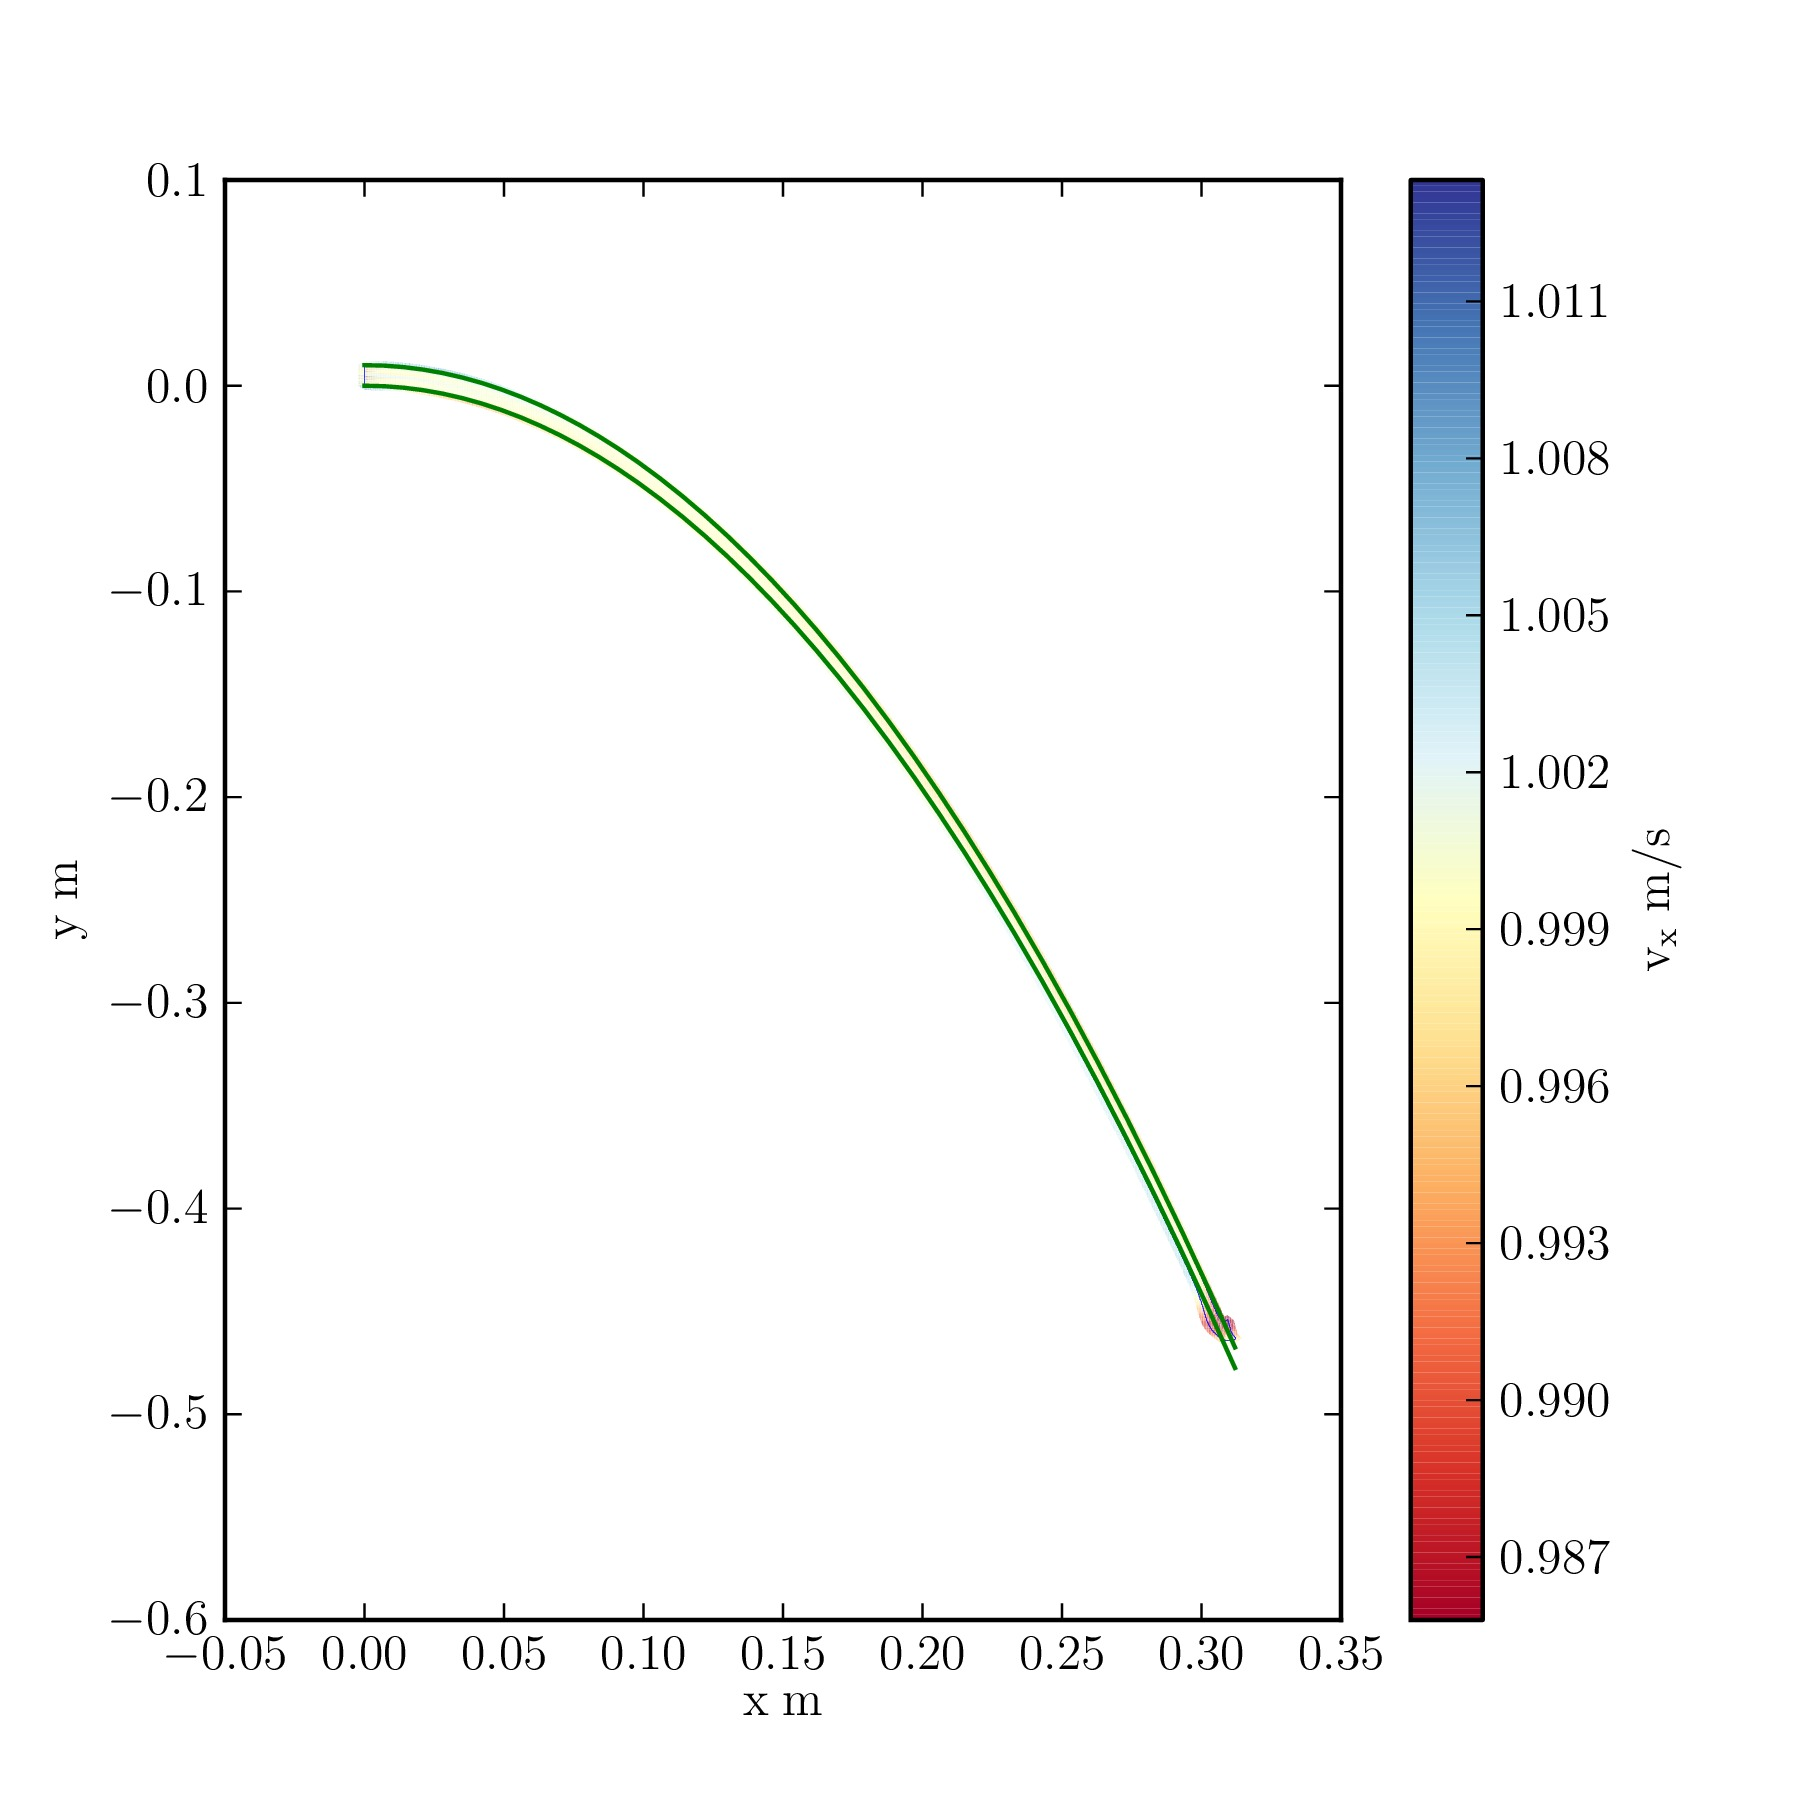
\includegraphics[width=0.8\textwidth]{plot_10__1_293.jpg}
\end{frame}

\begin{frame}{Jet latéral}
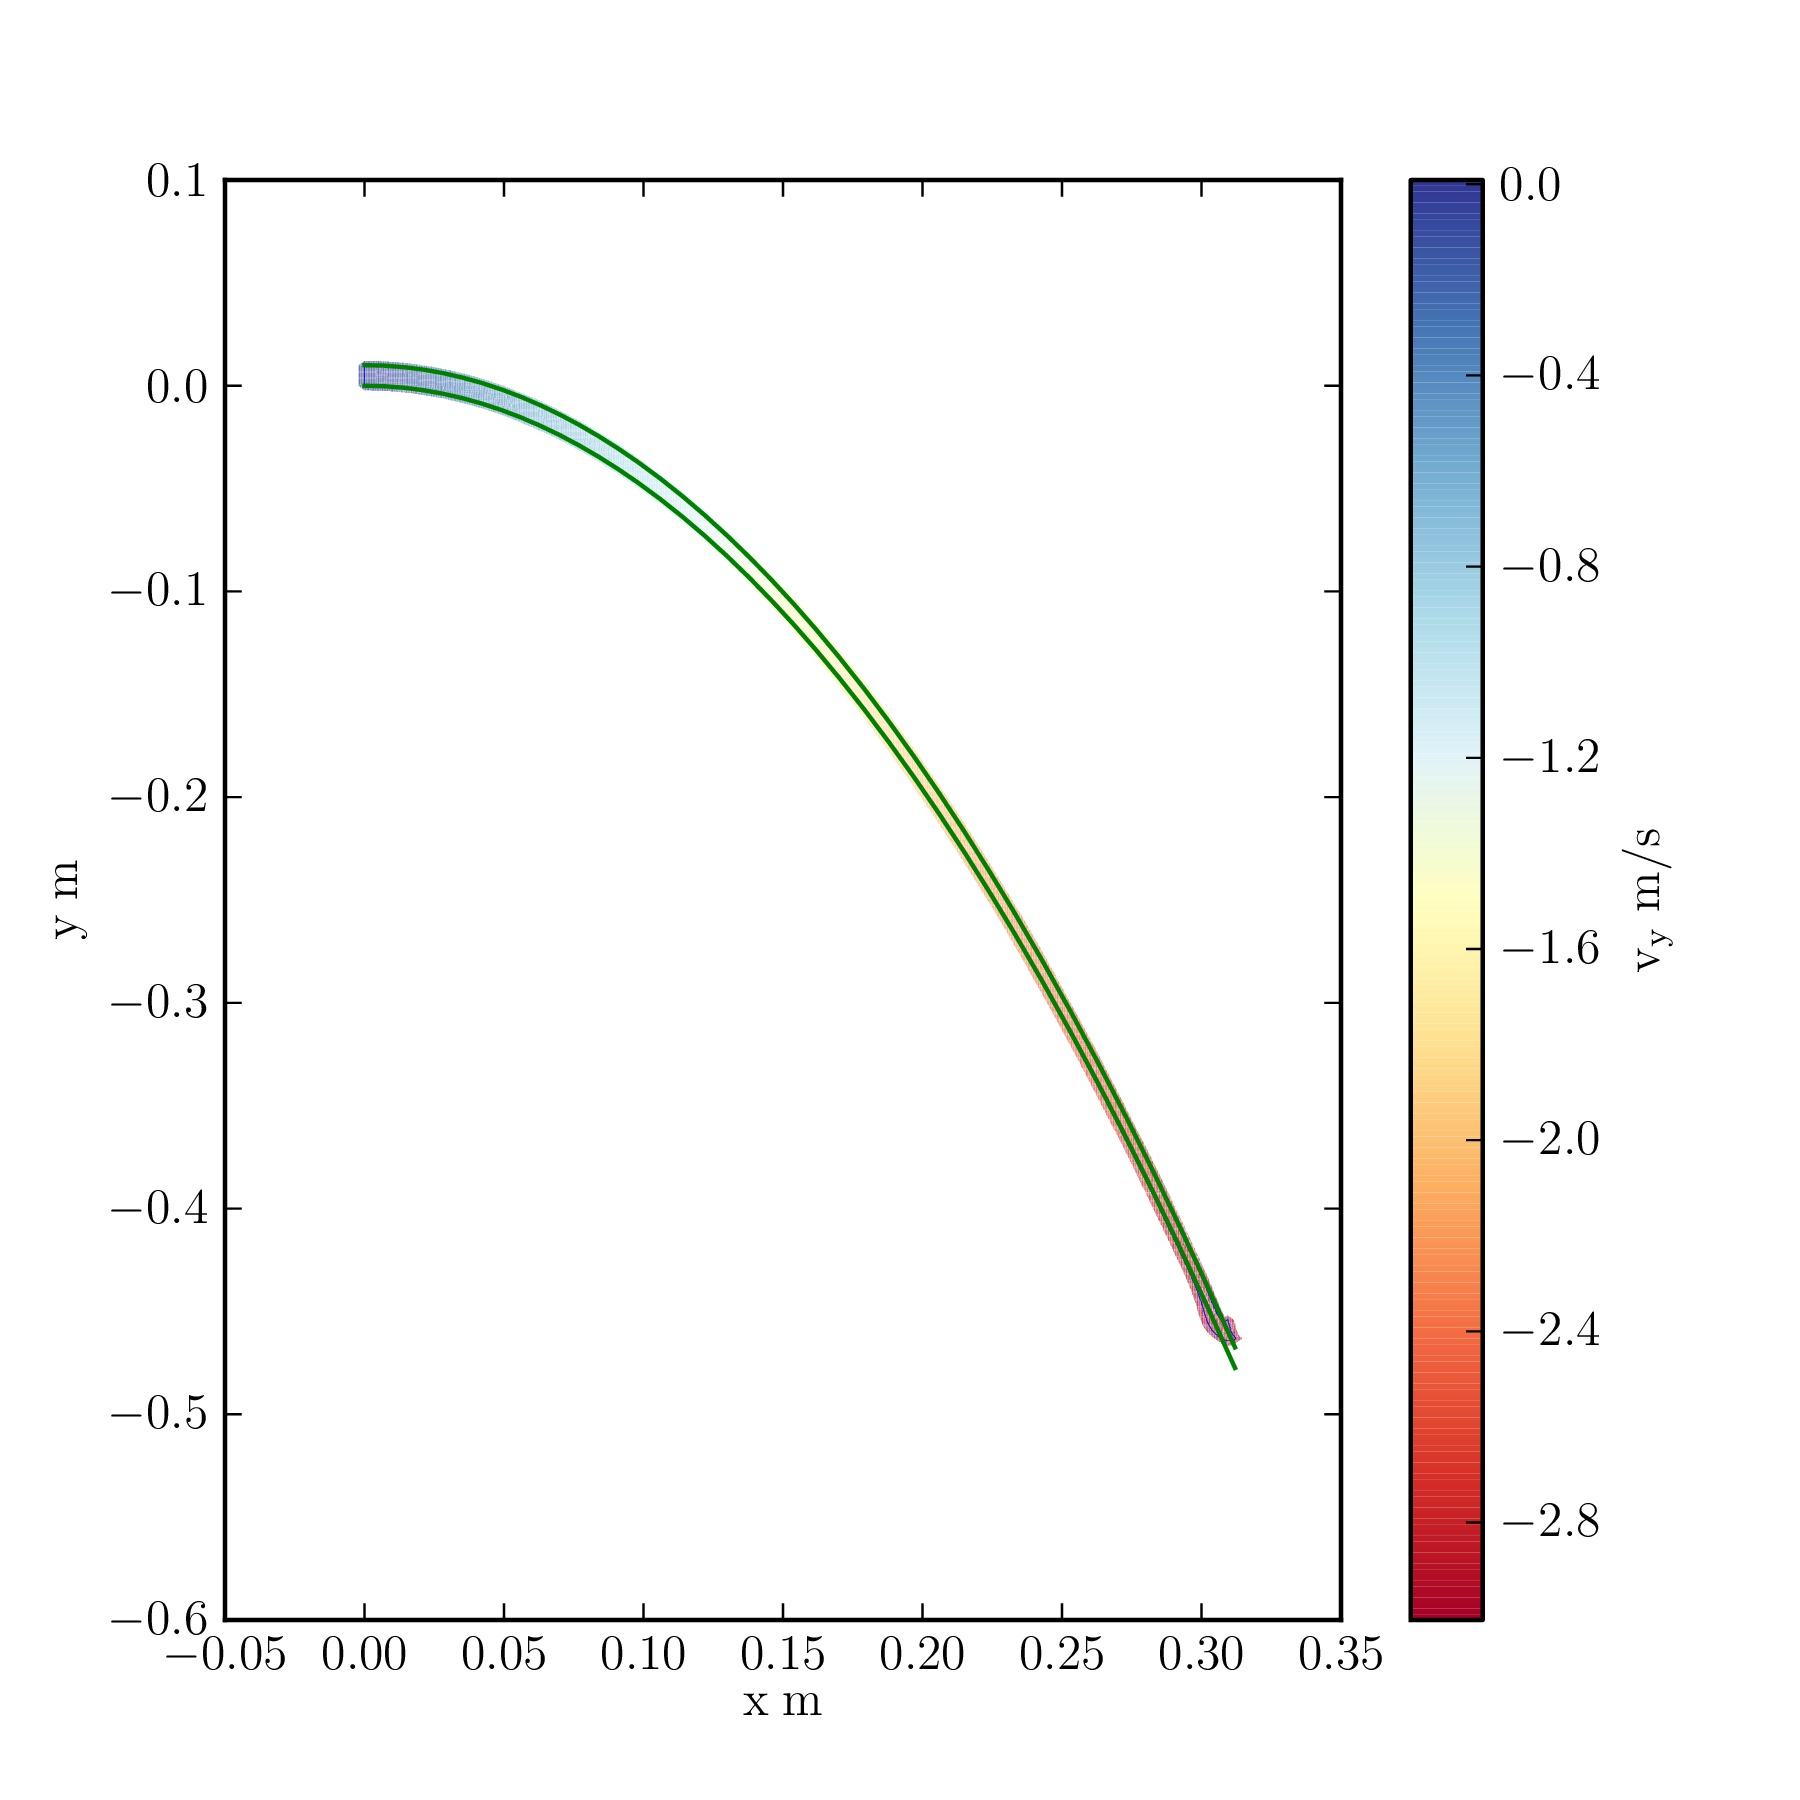
\includegraphics[width=0.8\textwidth]{plot_10__2_293.jpg}
\end{frame}

\begin{frame}{Jet latéral et Jet d'eau}

\end{frame}

 \section{Conclusion}

\begin{frame}[<+->]{Avantage et défaut}
 

  \begin{itemize}
   \plusitem Méthode de discrétisation bien connu.
   \plusitem Système linéaire facil à résoudre.
   \moinsitem Terme convectif plus dur.
   \plusitem Moins de voisin à traiter.
   \moinsitem Dépendant du choix des axes.
  \end{itemize}


 
\end{frame}

\begin{frame}[<+->]{Amélioration possible}
 
 \begin{block}<*>{MAC}
  \begin{itemize}
   \item Écrire une version parallèle du code.
   \item Solveur specialisé pour changement de topologie sans tout recalculer.
   \item Éviter l'effet escalier aux bords.
   \item Utiliser une autre forme de topologie que les particules.
   \item Ordre supérieur de discrétisation.
   \item Éviter le problème de saut dans les conditions aux bords.
  \end{itemize}
  \end{block}
 
\end{frame}

\begin{frame}{Remerciements}

\begin{block}{Personne}

\begin{description}
 \item[Prof. Martin Gander:] Pour m'avoir suivi dans ce travail ainsi que pour son cours d'analyse numérique.
 \item[Dr. Felix Kwok:] Pour m'avoir suivi dans ce travail et pour les tps et exercices.
 \item[Prof. Peter Wittwer:] Pour les cours de mathématiques et physique.
 \item[Reto, Norma, Roland, Tamara, Bruno, François:] Pour me soutenir et les bons moments passés ensemble.
\end{description}
 \end{block}
 \end{frame}
 
 \begin{frame}{Remerciements}
 \begin{block}{Logiciel}
  \begin{description}
   \item[Lua\LaTeX:] Pour l'écriture du rapport.
   \item[Gcc:] Pour compiler mon code c++11.
   \item[Valgrind:] Pour la détection des fuites memoires et autre érreurs de memoire.
   \item[Vtk:] Pour l'exportation des données.
   \item[Paraview:] Pour la visualisation des données.
   \item[Umfpacks:] Comme solveur linéaire directe.
   \item[Pyamg:] Comme solveur linéaire itératif.
   \item[Boost:] Pour contenir des librairies utiles comme Boost-Python utilisé comme binding avec Pyamg.
  \end{description}

 \end{block}

 
\end{frame}


\end{document}


